The BeRP ball is a weapons grade plutonium sphere used in detector and criticality experiments~\cite{BeRP_report}.
The ball represents a fission neutron source that is subcritical under normal conditions.
This tutorial features the bare BeRP ball with the SNAP detector~\cite{snapdetector} facing it on one side.

\begin{figure}[th]
  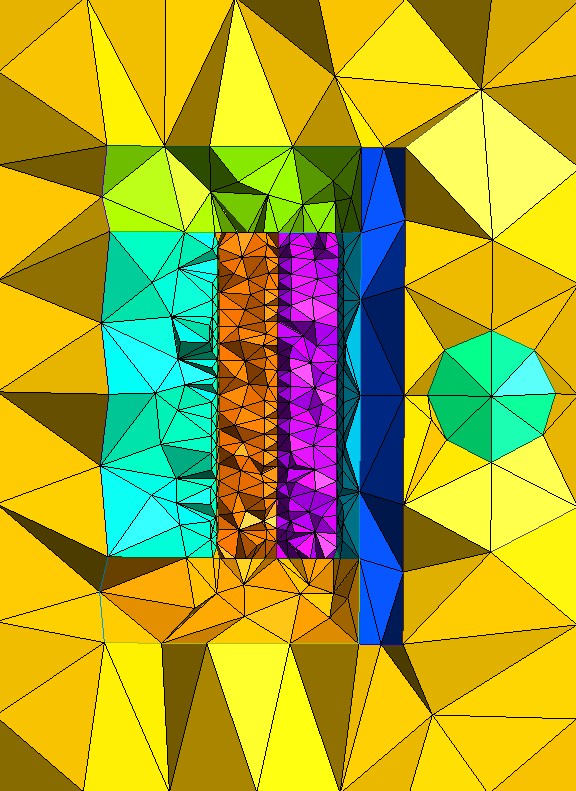
\includegraphics[height=1.0\textwidth, angle=90]{chapters/tutorials/figures/berp_snap_mesh.png}
  \caption{Mesh Slice for the Bare BeRP Ball with SNAP}
  \label{fig:berp_snap_mesh}
\end{figure}

This tutorial first explains how a tetrahedral mesh is created for the BeRP ball with SNAP detector, then the cross sections data input is discussed, the source specification is discussed, the standard input to THOR is covered, and finally the detector response calculation is shown.
The input files discussed below for the BeRP tutorial are located in:
\begin{verbatim}
    >> <thor_dir>/THOR/examples/tutorials/SNAP-BeRP
\end{verbatim}

\subsection{BeRP-SNAP Mesh}\label{ch:tuts:sec:berpsnap:ssec:mesh}

The workflow described here is suitable if the user has access to a compatible version of \href{https://gmsh.info/}{Gmsh}.
Any version 4 Gmsh should work, but the example specifically performed here was done using Gmsh version 4.10.1.

Begin by navigating to the location of the BeRP Gmsh geometry files, which are found in:
\begin{verbatim}
  <thor_dir>/THOR/examples/tutorials/SNAP-BeRP/mesh_create/
\end{verbatim}
Opening the file geometry file \verb"snap-berp.geo" in a text editor, construction of the BeRP and SNAP detector can be seen, as well as fields for differing mesh sizes for different regions.
For more details on creating original Gmsh inputs, see the \href{https://gmsh.info/doc/texinfo/gmsh.html}{Gmsh reference manual}.

Open \verb"snap-berp.geo" in Gmsh and run the ``3D'' command from the ``Mesh'' dropdown menu under ``Modules''.
The mesh should be generated and now become visible in the \ac{GUI}.
Now, select the ``Save'' command from the same ``Mesh'' dropdown to save the generated mesh to \verb"snap-berp.msh".
This mesh may be compared to the provided \verb"snap-berp_msh.ref", however they may differ slightly if the versions differ or if optimization of the mesh is employed.

The gmsh file \verb"snap-berp.msh" is converted to \ac{THOR}'s native mesh format by executing OpenMeshConverter with the command line:
\begin{verbatim}
  >> <thor_dir>/THOR/pre-processors/OpenMeshConverter/OpenMeshConverter.exe
      snap-berp.msh
\end{verbatim}
Note that since this is a full model, all sides of the boundary are set to the default (vacuum) (see Section~\ref{ch:getstart:sec:preproc:subsec:meshconv} for more details).
After successful completion of the conversion, the following printout should appear:
\begin{verbatim}
  ----------------------- Reading in gmsh:
  Progress:***********************************************************************
  ----------------------- Calculating Adjacencies:
  Progress:***********************************************************************
  ----------------------- Outputting thrm file:
  Progress:***********************************************************************
  ----------------------- Calculating volumes:
  Progress:***********************************************************************
  Region 1 tets: 46
  Region 1 volume:   1.7521346844666817E+02
  Region 2 tets: 510
  Region 2 volume:   1.2245928965492803E+03
  Region 9 tets: 224
  Region 9 volume:   5.1468066768394215E+02
  Region 10 tets: 215
  Region 10 volume:   5.1468066769054917E+02
  Region 11 tets: 178
  Region 11 volume:   1.0623536946432052E+03
  Region 12 tets: 523
  Region 12 volume:   1.2277835381550972E+03
  Region 13 tets: 45
  Region 13 volume:   4.2978526768381915E+00
  Region 14 tets: 45
  Region 14 volume:   4.2986387408112190E+00
  Region 15 tets: 214
  Region 15 volume:   2.1276304859489951E+01
  Region 16 tets: 217
  Region 16 volume:   2.1279857416591092E+01
  Region 17 tets: 141
  Region 17 volume:   1.3640485947888578E+01
  Region 18 tets: 137
  Region 18 volume:   1.3629468675220243E+01
  Region 19 tets: 2109
  Region 19 volume:   3.7255025368504766E+02
  Region 20 tets: 2142
  Region 20 volume:   3.7255520980715204E+02
  Region 21 tets: 1685
  Region 21 volume:   3.5669765582369166E+01
  Region 22 tets: 1685
  Region 22 volume:   3.5671727474747385E+01
  Region 23 tets: 1637
  Region 23 volume:   2.4515515354869885E+03
  Region 24 tets: 1580
  Region 24 volume:   4.5171458031465110E+04
  Region 25 tets: 955
  Region 25 volume:   2.5281620900188400E+02
  Total number of tets: 14288
  Total system volume:   5.3490000273988961E+04
  --------------------------------------------------------------------------------
  --------------------------------------------------------------------------------
  --------------------------------------------------------------------------------
  ------------------------- OpenMeshConverter successful -------------------------
  ----------------------- Output written to snap-berp_out.thrm
\end{verbatim}

The file \verb"snap-berp_out.thrm" should result from this execution for use by \ac{THOR}.
This mesh may be compared to the provided \verb"snap-berp_thrm.ref", which it should match if \verb"snap-berp.msh" matches \\
\verb"snap-berp_msh.ref".
Notice that the given volume for Region 1 (the BeRP sphere as seen in \verb"snap-berp.geo") is 175.2~cm$^3$, but the actual volume for the BeRP ball is 228.7~cm$^3$.
Similarly, the other regions meshed volumes also do not match their true volumes.
This concludes the mesh generation step for this tutorial.

\subsection{Cross section data}

The user should now move \verb"snap-berp_out.thrm" to the input file location
\begin{verbatim}
  <thor_dir>/THOR/examples/tutorials/SNAP-BeRP/
\end{verbatim}
and navigate there to continue the tutorial.

The \ac{THOR} cross section file for the BeRP benchmark is provided by \verb"snap-berp.xs".
\ac{THOR} uses a custom cross section format that is explained in detail in Section~\ref{ch:inp:sec:xsfile}.
These particular cross sections were generated using OpenMC~\cite{openmc} for the model shown and converted using the OpenXSConverter (see Sec.~\ref{ch:getstart:sec:preproc:subsec:xsconv}) included as a THOR submodule.

At the end of Section~\ref{ch:tuts:sec:berp:ssec:mesh}, it was observed that there was a discrepancy in the volume of the BeRP mesh compared to the original problem.
To preserve material mass, the cross sections must be altered by the ratio of the original volume to the meshed volume.
In \ac{THOR}, the user need not alter the cross sections themselves to make this adjustment.
Instead, \ac{THOR} will automatically adjust reaction and material attenuation calculations by a given density factor for each region.
By default, this factor is 1.0, which will lead to use of the original cross sections unaltered.
However, the user may specify density factors in a density factor file, described in Section~\ref{ch:inp:sec:densfact}.
For this tutorial, this density factor adjustment is provided by \verb"snap-berp.dens".
This file differs from the file in the Godiva tutorial in that it gives true region volumes instead of ratios of true to meshed volumes.
The effect is the same, however it is often simpler to specify the density factors in this manner since the density file will then need not be changed as the mesh is refined.

\subsection{Source specification}

The \ac{THOR} source file for the BeRP benchmark is provided by \verb"snap-berp.src".
\ac{THOR} uses a custom source format that is explained in detail in Section~\ref{ch:inp:sec:srcfile}.
Notice that mapping for source regions is not done (unlike cross section mapping), so the sources must be assigned to the proper source region in the source file compared to the THOR mesh.
For this problem that simply means source region 1 must be assigned all of the spontaneous fission source since OpenMeshConverter automatically assigns each cell matching region and source IDs, which for the BeRP spehere is region 1 as seen in \verb"snap-berp.geo".

\subsection{THOR input file and executing THOR}

The \ac{THOR} input file is \verb"snap-berp.inp".
\ac{THOR} uses a keyword-based input that is listed in Section~\ref{ch:inp:sec:stdinput}.
The SNAP-BeRP tutorial input file is not verbose and all parameters given are used, though not all are necessary since many are the same as the default values.
Upon running \ac{THOR}, a verbose form of the input will always be echoed, and ignored parameters will be highlighted as such.
\begin{verbatim}
  problem_type          fsrc
  lambda                0
  piacc                 errmode
  innerconv             1e-4
  outerconv             1e-4
  maxinner              4
  maxouter              50000
  pnorder               2
  mesh                  ./snap-berp_out.thrm
  density_factor        ./snap-berp.dens
  xs                    ./snap-berp.xs
  source                ./snap-berp.src
  qdtype                levelsym
  qdorder               8
  region_map            1  7
                        2  1
                        3  6
                        4  6
                        5  6
                        6  6
                        7  6
                        8  6
                        9  1
                        10 1
                        11 1
                        12 1
                        13 2
                        14 2
                        15 3
                        16 3
                        17 2
                        18 2
                        19 4
                        20 4
                        21 5
                        22 5
                        23 1
                        24 6
                        25 6
  vtk_flux_out          yes
  vtk_mat_out           yes
  vtk_src_out           yes
\end{verbatim}

The BeRP tutorial is solved with \ac{THOR} via the command line:
\begin{verbatim}
  >> mpirun -np 4 <thor_dir>/THOR/thor-1.0.exe snap-berp.inp
\end{verbatim}

Completion of execution of the SNAP-BeRP tutorial is indicated by the printout:
\begin{verbatim}
  --------------------------------------------------------
  Execution of THOR completed successfully
--------------------------------------------------------
\end{verbatim}

\ac{THOR} provides the following output that is discussed in this tutorial:
\begin{itemize}
    \item A summary of group-wise, region-averaged reaction rates is provided for each region identifier separately under ``Region averaged reaction rates''.
    The volume of each region, and group-wise fluxes, fission, absorption, and fission source rates are listed.
    Note that at the making of this tutorial, skipped region numbers are still printed with NaN fluxes.
    This will be fixed in the future.
    \item Three vtk formatted files, \verb"snap-berp_flux.vtk" contains spatial flux maps, \\
    \verb"snap-berp_mat.vtk" contains the material map, and \verb"snap-berp_src.vtk" contains the specified external source.
    These files can be opened with the \href{https://www.paraview.org/download/}{ParaView} post-processing tool.
\end{itemize}

A plot of the group 20 flux using ParaView 5.10.0 for this run is shown in Figure~\ref{fig:berp_g=20}.
\begin{figure}[th]
  \center
  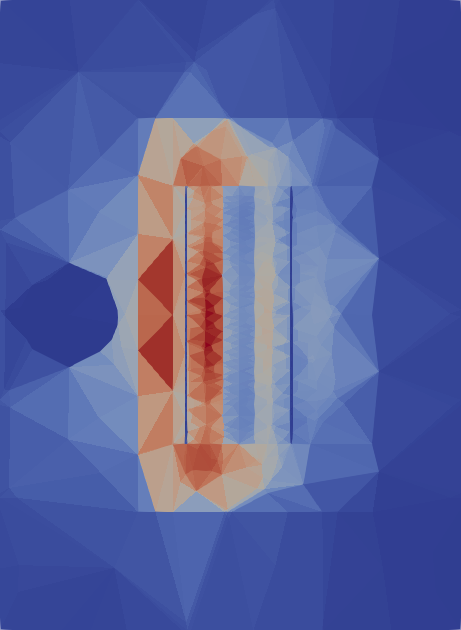
\includegraphics[height=1.0\textwidth, angle=-90]{chapters/tutorials/figures/berp_g=20.png}
  \caption{Group 20 flux for SNAP-BeRP tutorial.}
  \label{fig:berp_g=20}
\end{figure}

This tutorial concludes by showcasing how to compute a detector response using THOR's response calculation post-processors (see Sec.~\ref{ch:getstart:sec:preproc:subsec:respcalc}).
The response calculation input file is given in \verb"response_calc.in":
\begin{verbatim}
flux_files 1
snap-berp_flux.out
response_type region_wise
response_func response_function.resp
\end{verbatim}

The first line specifies the number of flux files to be summed up for response calculation, the second line gives the name for the flux file used in response calculation, the third line gives the type of detector response calculation, and the fourth gives the detector response function filename.
The detector response function file is given in \verb"response_function.resp".
In the detector response function file, the first line gives the THOR mesh file, the second line gives the number fo regions, and the third line onward gives the group-wise response function for each region.

For this response function, only regions 15 and 16 have non-zero response functions.
These regions are the two ``Active Helium'' regions of the SNAP detector and the response function given is the total Helium cross section which matches material 3 data in \verb"snap-berp.xs".
The response calculation can be performed using the following command:
\begin{verbatim}
  >> <thor_dir>/post-processors/THOR_Response_Calc/THOR_Response_Calc.exe response_calc.in
\end{verbatim}
This will give a total response of 2.07 to both the terminal and \verb"response_calc.in_response.out".
This result should match almost exactly with the value in \verb"response_calc_in_response_out.ref".
Note that the total flux, and therefore also this response, is proportionate to the total source given for a fixed source problem.
So if it is to be compared to response per NPS from a Monte Carlo code, it must be divided by the integrated specified fixed source.

Notice that in the region summary at the end of the THOR output, region 15 is given volume 2.127630E+01 cm$^3$ and spatially averaged absorption rate 5.355295E-02 $\frac{\text{abs}}{\text{s-cm}^3}$ for a total absorption rate of $1.139~\frac{\text{abs}}{\text{s}}$ while region 16 has a given volume of 2.127986E+01 cm$^3$ and spatially averaged absorption rate of 1.364049E+01 $\frac{\text{abs}}{\text{s-cm}^3}$ for a total absorption rate of $0.919~\frac{\text{abs}}{\text{s}}$.
So the combined total absoprtion rate for the two regions is $2.05~\frac{\text{abs}}{\text{s}}$, which is close to our computed response.
The difference betwen this value and our computed response comes from a combination of the fact that the response calculator is computing total reaction rate while the THOR region summary reports just absorption rate, and the fact that the THOR region report uses cross sections that have been scaled using the density factors while the response calculation does not.

The results can be improved by increasing the refinement of the mesh and convergence criteria in the THOR input file.